\section{Conclusion, Limitations \& Future Work}
\label{sec:limitations}

\paragraph{Conclusion}
In summary, our method demonstrates the effectiveness of combining reconstruction techniques with an object-level generation framework to significantly enhance the aesthetic quality of 3D instances within a reconstructed scene.
Moreover, our approach facilitates a straightforward process for generating virtual environments from single images, with potential applications in gaming, virtual reality, and augmented reality settings.
An additional advantage of utilizing a multi-modal diffusion model instead of directly leveraging high-quality 3D objects, such as CAD models, is the ability to customize inputs, enabling fine-grained control over the reconstructed scene.

\paragraph{Limitations}
While our results show promise, it's important to acknowledge certain limitations of our method.
Firstly, concerns arise regarding object detection.
While the panoptic reconstruction model doesn't necessarily need to detect an instance to reconstruct its approximate shape, SDFusion is only applied to detected objects.
As a result, undetected objects and instances erroneously identified as part of another object may be entirely omitted from the refinement process.
Moreover, noisy instance segmentations pose another challenge, as our scale and position estimations are contingent upon the predicted instance labels.
Hence, instance segmentations that include parts of other instances or elements of the surrounding environment can lead to the creation of larger, misplaced refined instances.
A concrete example of this phenomenon is presented in \cref{fig:lim}.

\begin{figure}[t]
  \centering
  \begin{subfigure}{0.3\linewidth} % Adjust the width for three images in one row
    \centering
    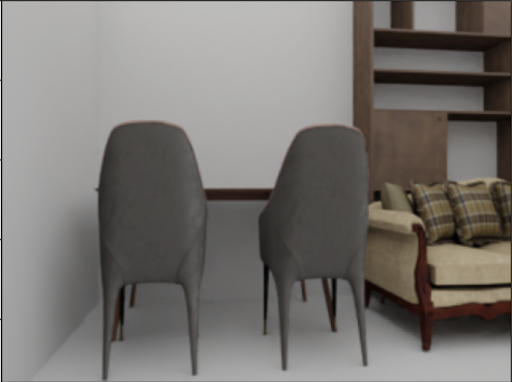
\includegraphics[width=\linewidth]{figs/inputlim.png}
    \caption{Input Image}
    \label{subfig:limsub1}
  \end{subfigure}
  \hspace{0.02\linewidth} % Adjust spacing between figures
  \begin{subfigure}{0.3\linewidth} % Adjust the width for three images in one row
    \centering
    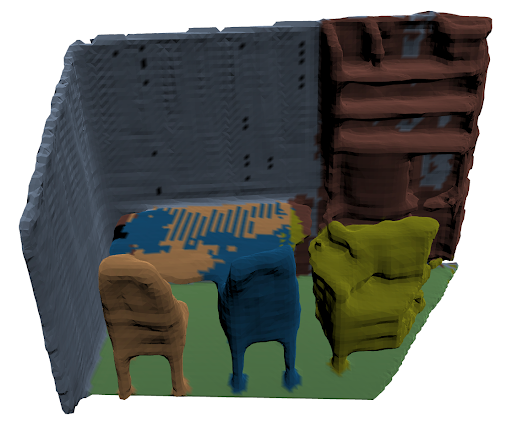
\includegraphics[width=\linewidth]{figs/panolim.png}
    \caption{Initial Scene Reconstruction}
    \label{subfig:limsub2}
  \end{subfigure}
  \hspace{0.02\linewidth} % Adjust spacing between figures
  \begin{subfigure}{0.3\linewidth} % Adjust the width for three images in one row
    \centering
    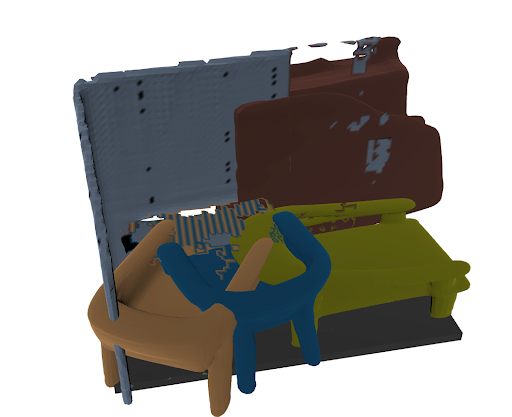
\includegraphics[width=\linewidth]{figs/ourslim.png}
    \caption{Final Output}
    \label{subfig:limsub3}
  \end{subfigure}

  \caption{Our method struggles with missing and ambiguous semantic/instance labels. As the initial instance segmentation fails to identify the 'Table' object, the corresponding geometry is entirely absent from our reconstruction. Furthermore, since the 'Chair' instance masks overlap with the table geometry, our method generates corresponding instances with incorrect scale and pose.}
  \label{fig:lim}
\end{figure}
\vspace*{-5mm}

\paragraph{Future Work}
\label{sec:future}
To overcome these limitations, we suggest two avenues for future research.
The first direction involves implementing end-to-end training with adapted loss functions, aimed at penalizing misidentified instances more effectively.
This approach could enhance the accuracy of instance segmentation and reduce the incidence of missing or misattributed objects in the reconstructed scene.
Secondly, refining the merging process by integrating a pose estimation network can be utilized to enhance object alignment and scaling.
Another promising avenue for exploration involves guiding object-level reconstruction with more detailed descriptive inputs.
By incorporating these object descriptions during inference -- inspired by the findings of the SDFusion paper -- we can potentially generate more tailored and contextually relevant reconstructions.
% We conducted separate training for both the Panoptic model and the SDFusion model. To increase the performance we advocate for an end-to-end training approach. Given that the Panoptic model outputs occupancies and a distance field in terms of geometry, a differentiable transformation to a signed distance field is necessary to allow end-to-end training. This integration would enable SDFusion to effectively backpropagate gradients and directly learn from SDFusion's noisy inputs. Another constraint lies in our registration algorithm, which selects one out of 16 predefined positions, which can pose a challenge in achieving perfect alignment relying on the initial orientation of the reconstructed objects. A more robust alignment strategy can enhance the overall quality of the final scene.